\chapter{Fundamentos teóricos}
\pagenumbering{arabic}

\section{Redes neuronales recurrentes de tiempo continuo (CTRNN)}
En contraste con las redes neuronales feed-forward, las cuales soportan únicamente comportamientos
reactivos, en las Redes Neuronales Recurrentes de Tiempo Continuo (CTRNN) \cite{BeerRD}
pueden existir ciclos en su estructura y la activación de sus neuronas es asíncrona y multiescalada
en el tiempo. Este tipo de redes neuronales también facilita describir el agente como un
sistema dinámico acoplado al entorno en el que está ubicado, ya que está demostrado que son el
modelo más simple de red neuronal dinámica continua no lineal \cite{FunaYNaka}
Además, la interpretación neurobiológica de las CTRNN ha sido demostrada y puede consultarse
en \cite{BeerRD}.

\subsubsection{Descripción matemática de una CTRNN}
Las CTRNN están formadas por neuronas cuyo comportamiento se describe en las ecuaciones \ref{eq:funcionCTRNN} y \ref{eq:funcionSIGMOIDE}
\begin{equation} \label{eq:funcionCTRNN}
	\dot{y_{i}}= \frac{1}{\tau_{i}} * \left ( -y_{i}+\sum_{j=1}^{N}w_{ji}*\sigma \left ( y_{j} + \theta _{j} \right ) + I_{i} \right ) \qquad i =1,2,...,N
\end{equation}
\begin{equation} \label{eq:funcionSIGMOIDE}
	\sigma (x)=\frac{1}{1+e^{-x}}
\end{equation}
donde $y_{i}$ es el estado de la neurona, $w_{ji}$ es el peso de la conexión entre las neuronas i y j,
$\theta$ es el término bias, I representa una entrada externa y $\tau$ hace que cada una de las neuronas
dependa del tiempo, ya que para diferentes valores la caída del nivel de activación de la neurona
es más rápida o lenta. En la fórmula \ref{eq:funcionCTRNN} la velocidad de actualización de la red neuronal debe ser
notablemente mayor (el intervalo entre dos actualizaciones será menor) que el valor de $\tau$ para no
obtener comportamientos no deseados.

\subsubsection{Valores de activación y de salida de la neurona de una CTRNN}
Para poder entender cómo deben interpretarse la activación y la salida de una CTRNN, se va
a utilizar como ejemplo una CTRNN formada por una única neurona autoconectada como la de la figura \ref{fig:figuraCTRNNBasica}.
El valor de salida o de una neurona será un valor real entre 0 y 1 obtenido al aplicar la función
sigmoide (ecuación \ref{eq:funcionSIGMOIDE}) a la suma del estado actual y de la neurona con su valor bias $\theta$, tal y
como puede verse en la figura \ref{fig:figuraCTRNNBasica}.
\begin{figure}[H]
    \centering
    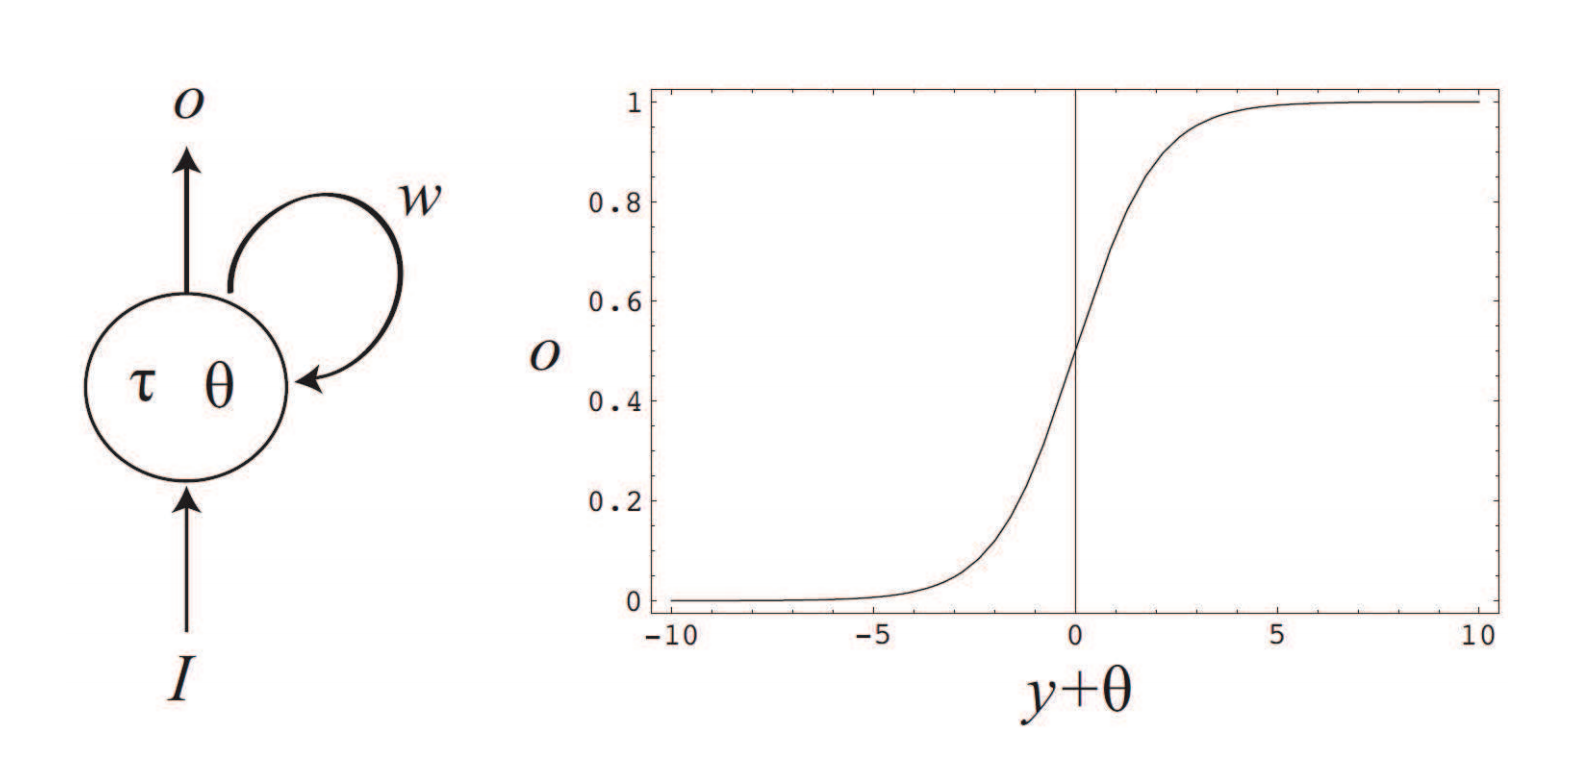
\includegraphics[width=0.8\textwidth,height=6cm]{Imagenes/CTRNNBasica}
    \caption{Valor de salida de una CTRNN. \textbf{Izquierda:} Un nodo autoconectado. \textbf{Derecha:} Función sigmoide aplicada para calcular la salida de una neurona.}
    \label{fig:figuraCTRNNBasica}
\end{figure}

En cuanto al valor de activación, a diferencia de una red neuronal feed-forward, la cual realiza
un mapeo directo entre entrada y salida de la red, el comportamiento de una CTRNN corresponde
al de un sistema dinámico \cite{BeerRD}, por lo que el valor de activación de la neurona convergerá
a un punto de equilibrio. Para el análisis de las dinámicas del sistema formado por el agente
controlado por la CTRNN y el entorno, se analizarán sus diagramas de bifurcación, los cuales
muestran todos los puntos de equilibrio para la activación de las neuronas de la red.

\section{Homeostasis}
A pesar de que la homeostasis es una propiedad biológica, es posible representar un sistema lógico que se comporte de forma similar a como
sistemas vivos con estas propiedades lo harían\cite{Hywel}.

Un \textit{Homeostato}, es un sistema artificial que presenta porpiedades de homeostasis. El Homeostato desarrollado por Ashby era un aparato
electromagnético mientras que el que va a ser utilizado es un componente implementado computacionalmente.

Un Homeostato es un sistema de $N$ neuronas completamente interconectadas entre si. Cada neurona recibe $N$ entradas, de si misma y del resto de neuronas,
dependientes del peso de la fuerza de conexión de las uniones entre ellas (ver Figura \ref{fig:figuraHomeostatSchema}).

\begin{figure}[!h]
    \centering
    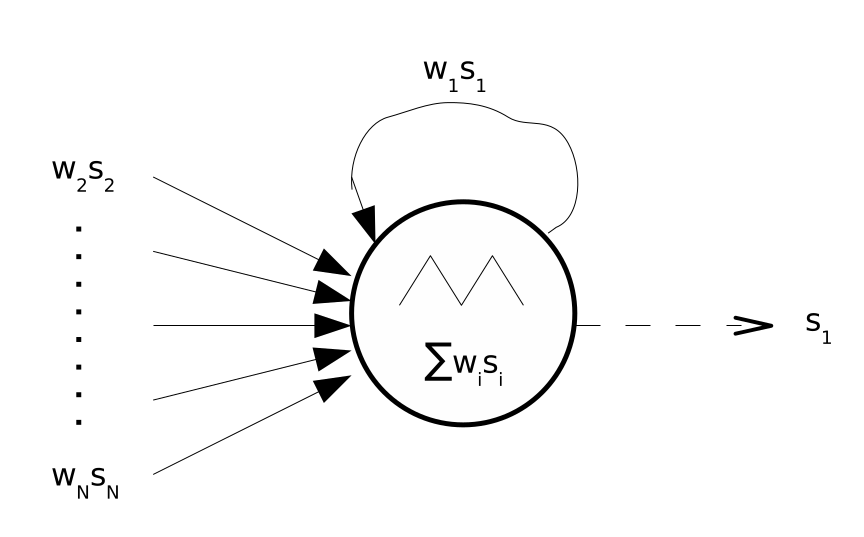
\includegraphics[width=0.6\textwidth,height=5cm]{Imagenes/HomeostatSchema}
    \caption{Esquema de un Homeostato individual. La unidad recibe las entradas del resto de unidades ($w_{i}s_{i}$) y de si misma ($w_{1}s_{1}$). La salida $s_{1}$ es una función lineal por partes
		de la suma ponderada de las entradas.)}
    \label{fig:figuraHomeostatSchema}
\end{figure}

\begin{figure}[!h]
    \centering
    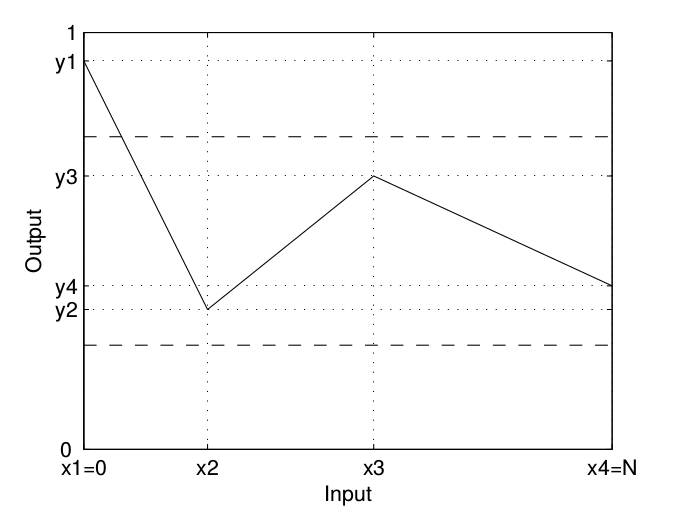
\includegraphics[width=0.6\textwidth,height=6cm]{Imagenes/HomeostatTransfer}
    \caption{Ejemplo de función de transferencia de una unidad Homeostat. La función es lineal por partes con puntos en ($x_{1},j_{1}$),...,($x_{p},y_{p}$) donde $x_{1}$ = 0 y $x_{p}$ = $N$, para todas las
		unidades en una red de $N$ unidades. Las líneas discontinuas representan el rango homeostatico de la red.}
    \label{fig:homeostatTransferFunction}
\end{figure}

La suma ponderada $I$ (ver ecuación \ref{eq:sumaPonderadaHomeostat}) de las entradas de una unidad determina su salida $s$, tal y como está especificado por la función linear de transferencia por
partes $F$ (ecuación \ref{eq:ecuPartesHomeostat} y figura \ref{fig:homeostatTransferFunction}).

\begin{equation} \label{eq:sumaPonderadaHomeostat}
	I = \sum_{i}^{N}w_{i}s_{i}
\end{equation}

\begin{equation} \label{eq:ecuPartesHomeostat}
	s = F(I)=\begin{cases}
y_{1}+(y_{2}-y_{1})(\frac{I-x_{1}}{x_{2}-x_{1}}) & \text{ : }\quad x_{1} \leq I < x_{2} \\
y_{2}+(y_{3}-y_{2})(\frac{I-x_{2}}{x_{3}-x_{2}}) & \text{ : }\quad x_{2} \leq I < x_{3} \\
y_{3}+(y_{4}-y_{3})(\frac{I-x_{3}}{x_{4}-x_{3}}) & \text{ : }\quad x_{3} \leq I \leq  x_{4} \\
\end{cases}
\end{equation}

Al inicializar la red, los pesos de las conexiones se aleatorizan a partir de una distribución uniforme de rango apropiado. El rango objetivo (o rango límite) $R = [0.5 - \delta, 0.5 + \delta]$ es
especificado para la salida, donde $\delta$ determina la rigidez de la restricción homeostática. Si $s \in R$ la unidad es homeostática. Si $s \notin R$ significa que la homeostasis se ha perdido
y se activan los mecanismos de cambio adaptativo.

Hay dos mecanismos de cambio adaptativo que se aplican a los parámetros de las unidades no homeostáticas. El primer mecanismo asigna valores aleatorios a los pesos de las conexiones aferentes a la unidad (ecuación \ref{eq:aferenteEQ}).
El segundo mecanismo asigna nuevos valores aleatorios a los parámetros que indican las coordenadas de la función de transferencia de la unidad (ecuación \ref{eq:transferEQ}). Los rangos de estas reasignaciones son los mismos utilizados
en la inicialización. Donde $rand(a,b)$ representa a la función que devuelve un número real aleatorio obtenido de una distribución uniforme en el rango $[a,b]$.

\begin{equation} \label{eq:aferenteEQ}
	\text{\textit{IF}} \quad (s \notin R) \quad \text{\textit{THEN}} \quad [w= \text{\textit{rand}}(0.00, 1.00) \quad \forall w \in \left \{ w_{1},...,w_{N} \right \}]
\end{equation}

\begin{equation} \label{eq:transferEQ}
	\begin{aligned}
	 \text{\textit{IF}} \quad (s \notin R) \quad \text{\textit{THEN}} \quad [x= \text{\textit{rand}}(0.00, N) \quad \forall x \in \left \{ x_{2},...,x_{p-1} \right \}]& \\
	 \qquad \qquad \qquad \,\quad  \text{\textit{AND}} \quad [y= \text{\textit{rand}}(0.00, 1.00) \quad \forall y \in \left \{ y_{1},...,y_{p} \right \}]& \\
 \end{aligned}
\end{equation}

Durante la realización de este trabajo de diseñó e implementó un sencillo Homeostato para comprender mejor los fundamentos que lo definen. La descripción de este Homeostato puede encontrase en el Anexo \ref{ch:anexo1} y puede servir como
ejemplo sencillo para ayudar a comprender los fundamentos de la homeostasis.


\section{Algoritmo genético}
Los algoritmos genéticos son un método para resolver problemas de optimización. Estos algoritmos están basados en la selección natural, que es el proceso que dirige la evolución biológica. Un algoritmo genético modifica repetidas veces
una poblacion de posibles soluciones. En cada iteración, se seleccionan las mejores posibles soluciones encontradas hasta el momento y se genera a partir de ellas una nueva generación de candidatos. Generación tras generación la
población evoluciona hacia la solución óptima.

Los algoritmos genéticos difieren de los los algoritmos clásicos de optimización en tres puntos principales:
\begin{enumerate}
	\item{Los algoritmos clásicos generan un único punto con cada iteración mientras que los algoritmos genéticos generan una población de puntos con cada iteración.}
	\item{En los algoritmos clásicos la secuencia de puntos se aproxima en cada iteración a la solución óptima mientras que en los algoritmos genéticos es el mejor punto de la población el que se aproxima a la solución óptima.}
	\item{Los algoritmos clásicos generan el siguiente punto de la secuencia mediante un cálculo determinista mientras que los algoritmos genéticos selecciona el siguiente punto en la secuencia mediante cálculos que utiliza generadores de números aleatorios.}
\end{enumerate}

Una descripción más detalla de los algoritmos genéticos, tanto de su funcionamiento como de las partes que lo componen, puede encontrarse en el Anexo \ref{ch:anexo2}.
